
\begin{frame}
    \frametitle{Geometric approach}
    \begin{textblock*}{70mm}(8mm, 19mm)
        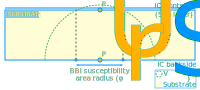
\includegraphics[width=\textwidth]{geomCrossViewNew.pdf}
    \end{textblock*}
    \begin{textblock*}{70mm}(83mm, 22.522mm)
        \includegraphics[width=\textwidth]{geomCrossViewThinNew.pdf}
    \end{textblock*}
    \begin{textblock*}{100mm}(29mm, 60mm)
        \centering
        \begin{equation*}
            \phi_r(t) = 2 \cdot \sqrt{r(t)^2 - t^2_{SUB}}
        \end{equation*}
        \begin{equation*}
            \frac{\phi_r^{THIN}}{\phi_r^{THICK}} = \sqrt{\frac{r^2 - t^2_{THIN}}{r^2 - t^2_{THICK}}} > 1
        \end{equation*}
        Higher susceptibility area → greater current density
    \end{textblock*}
\end{frame}

\begin{frame}
    \frametitle{Geometric approach}
    \begin{textblock*}{70mm}(8mm, 19mm)
        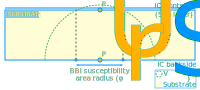
\includegraphics[width=\textwidth]{geomCrossViewNew.pdf}
    \end{textblock*}
    \begin{textblock*}{70mm}(83mm, 22.522mm)
        \includegraphics[width=\textwidth]{geomCrossViewThinNew2.pdf}
    \end{textblock*}
    \begin{textblock*}{100mm}(29mm, 60mm)
        \vspace{7mm}
        \centering
        \begin{equation*}
            \label{chap4:sect:geomModel:eqnVpu*}
            V_{PU}^* = \frac{t_{THIN}}{t_{THICK}} \cdot V_{PU} + V_F \cdot (1 - \frac{t_{THIN}}{t_{THICK}})
        \end{equation*}
    \end{textblock*}
\end{frame}

\begin{frame}{Geometric approach outcomes}
    \begin{itemize}
        \setlength\itemsep{2em}
        \item Thinning the substrate → Reduce the voltage pulse for a given susceptibility area
        \item Thinning the substrate → Susceptibility area increases at constant voltage
        \item Thinning the substrate → No improvement in resolution
    \end{itemize}
\end{frame}
